\model{Reference Types}

\begin{quote}
\begin{multicols}{2}

\begin{javalst}
int count;
double price;
String name;
Scanner in;

count = 0;
price = 1.99;
name = "Beyonce";
in = new Scanner(System.in);
\end{javalst}

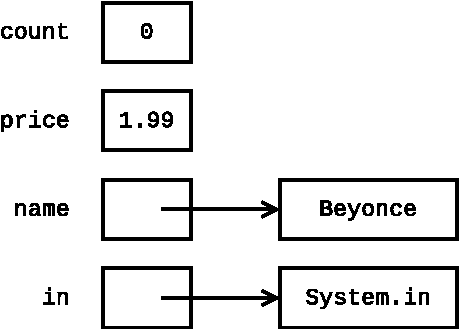
\includegraphics[width=\linewidth]{reference1.pdf}

\end{multicols}
\end{quote}

Java has eight primitive types (see \ref{primitive-types}).
All other types of data are called \emph{reference} types, because \textbf{their value is a memory address}.
When drawing state diagrams, use an arrow to \emph{reference} other memory locations (rather than make up integer values for the actual addresses).


\quest{15 min}


\Q What are the reference types in the example above?

\begin{answer}
String and Scanner
\end{answer}


\Q By convention, what is the difference between primitive and reference type names?

\begin{answer}
Primitive types are lowercase, and reference types are capitalized.
\end{answer}


\Q Variables in Java can use at most eight bytes of memory. Explain why \java{"Beyonce"} and \java{System.in} cannot be stored directly in the memory locations for \java{name} and \java{in}.

\begin{answer}
Both values are much larger than eight bytes, so they need to be stored somewhere else.
\end{answer}


\Q What is the value of the variable \java{count}? What is the value of the variable \java{price}?

\begin{answer}
The values are 0 and 1.99. They are stored directly in the variable's memory.
\end{answer}


\Q What is the value of the variable \java{name}? What is the value of the variable \java{in}?

\begin{answer}
The values are memory addresses. They reference the location where the actual data is stored.
\end{answer}


\Q \label{assign} Carefully explain what it means to assign one variable to another. For example, what does the statement ~ \java{price = count;} ~ do in terms of memory?

\begin{answer}
Assignment simply copies the value of one variable to another.
In the case of reference types, it only copies the memory location.
\end{answer}


\Q Draw a state diagram for the following code. Make sure your answer is consistent with what you wrote for \ref{assign}.

\begin{multicols}{2}

\begin{javalst}
int width;
double score;
Scanner input;
String first;
String other;

width = 20;
score = 0.94;
input = new Scanner(System.in);
first = "Taylor";
score = width;
other = first;
\end{javalst}

\columnbreak

\begin{answer}[3in]
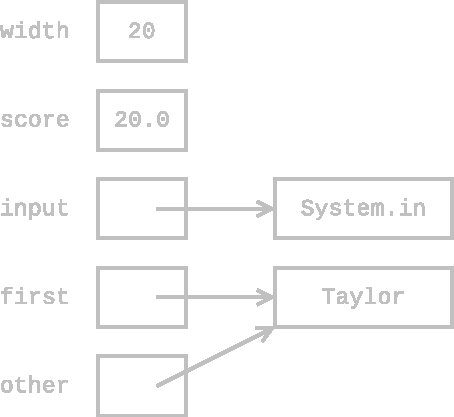
\includegraphics{reference2.pdf}
\end{answer}

\end{multicols}


\Q What is the output of the following statements after running the code above?
Explain your answer using the diagram.

\begin{javalst}
first = "Swift";
System.out.println(other);
\end{javalst}

\begin{answer}
Taylor, because changing the value (i.e., reference) of \java{first} does not affect the value of \java{other}.
\end{answer}
